\documentclass{article}

%%%%%%%%%%%%%%%%%%%%%%%%%
% Packages & Macros
%%%%%%%%%%%%%%%%%%%%%%%%%

% For including graphics
\usepackage{graphicx}

% For title page
\usepackage{datetime}
\newdateformat{monthyeardate}{\monthname[\THEMONTH] \THEYEAR}

% For supporting linking
\usepackage{hyperref}
\hypersetup{colorlinks,urlcolor=blue,linkcolor=blue,anchorcolor=blue,citecolor=blue}

% For table colouring (in command line tables)
\usepackage{colortbl}

% For supporting subfigure captions
\usepackage{subcaption}

% Allow paragraphs to be numbered
\setcounter{secnumdepth}{4}

%%%%%%%%%%%%%%%%%%%%%%%%%
% Tool-Specific Macros
%%%%%%%%%%%%%%%%%%%%%%%%%
\usepackage{xspace}

\newcommand{\args}[1] {\textit{#1}}
\newcommand{\cmd}[1] {\texttt{#1}}     % Use for command window commands, e.g., \cmd{svn up}
\newcommand{\block}[1] {\textsf{#1}}   % Use for Simulink block names, e.g., \cmd{Subsystem1}
\newcommand{\signal}[1] {\textsf{#1}}   % Use for Simulink block names, e.g., \cmd{Subsystem1}
\newcommand{\ring}[1] {\textsf{#1}} 	 % Use for files names and paths
\newcommand{\keyword}[1] {\texttt{#1}} % Use for keywords of programming languages, e.g., \keyword{while}
\newcommand{\file}[1] {\texttt{#1}} 	 % Use for files names and paths
\newcommand{\param}[1] {\textsf{#1}}   % Use for block parameter names, e.g., \param{BlockType}

% Matlab Products
\newcommand{\matlab}{\textsc{Matlab}\@\xspace}
\newcommand{\Matlab}{\textsc{Matlab}\@\xspace}
\newcommand{\Simulink}{Simulink\@\xspace}
\newcommand{\simulink}{Simulink\@\xspace}
\newcommand{\SDV}{Simulink Design Verifier\@\xspace}
\newcommand{\mpath}{\Matlab search path\@\xspace}

% Block Names (not BlockType)
\newcommand{\ds}{\block{Data Store}\@\xspace}
\newcommand{\DSM}{\block{Data Store Memory}\@\xspace}
\newcommand{\DSR}{\block{Data Store Read}\@\xspace}
\newcommand{\DSW}{\block{Data Store Write}\@\xspace}
\newcommand{\DSRW}{\block{Data Store Read/Write}\@\xspace}
\newcommand{\DSMRW}{\block{Data Store Memory/Read/Write}\@\xspace}

\newcommand{\goto}{\block{Goto}\@\xspace}
\newcommand{\from}{\block{From}\@\xspace}

\newcommand{\inport}{\block{Inport}\@\xspace}
\newcommand{\outport}{\block{Outport}\@\xspace}
\newcommand{\constant}{\block{Constant}\@\xspace}
\newcommand{\ground}{\block{Ground}\@\xspace}
\newcommand{\subsystem}{\block{Subsystem}\@\xspace}

\newcommand{\logic}{\block{Logical Operator}\@\xspace}
\newcommand{\relational}{\block{Relational Operator}\@\xspace}
\newcommand{\ifblk}{\block{If}\@\xspace}
\newcommand{\switch}{\block{Switch}\@\xspace}
\newcommand{\merge}{\block{Merge}\@\xspace}

\newcommand{\docblock}{\block{DocBlock}\@\xspace}

\newcommand{\simfunc}{\block{Simulink Function}\@\xspace}
\newcommand{\simfunccaller}{\block{Function Caller}\@\xspace}

\newcommand{\toworkspace}{\block{To Workspace}\@\xspace}
\newcommand{\fromworkspace}{\block{From Workspace}\@\xspace}

\newcommand{\tofile}{\block{To File}\@\xspace}
\newcommand{\fromfile}{\block{From File}\@\xspace}

\newcommand{\fromspreadsheet}{\block{From Spreadsheet}\@\xspace}

\newcommand{\modelref}{\block{Model Reference}\@\xspace}
\newcommand{\library}{\block{Library}\@\xspace}
\newcommand{\librarylink}{\block{Library Link}\@\xspace}

% Commonly used parameters
\newcommand{\AND}{\param{AND}\@\xspace}
\newcommand{\OR}{\param{OR}\@\xspace}
\newcommand{\NOT}{\param{NOT}\@\xspace}
\newcommand{\NOR}{\param{NOR}\@\xspace}
\newcommand{\NAND}{\param{NAND}\@\xspace}
\newcommand{\XOR}{\param{XOR}\@\xspace}
\newcommand{\NXOR}{\param{NXOR}\@\xspace}

% Common Abbreviations
% Example
\newcommand{\eg}{\textrm{e.g.,}\@\xspace}

% That Is To Say
\newcommand{\ie}{\textrm{i.e.,}\@\xspace}

% And So On
\newcommand{\etc}{\textrm{etc.}\@\xspace}

% And Others
\newcommand{\etal}{\textrm{et al.}\@\xspace}

% With Respect To
\newcommand{\wrt}{\textrm{w.r.t.}\@\xspace}

% Vice Versa
\newcommand{\vrsa}{\textrm{vice versa}\@\xspace}

% Symbols

\usepackage{amssymb}
\newcommand{\checkbox}{\makebox[0pt][l]{$\square$}\raisebox{.15ex}{\hspace{0.1em}$\checkmark$}}%
\newcommand{\uncheckbox}{$\square$~}%


\newcommand{\ToolName}{Auto Layout Tool\@\xspace}

\newcommand{\menu}[1]{%
	\ifthenelse{\equal{#1}{1}}{Auto Layout}{}%
  	\ifthenelse{\equal{#1}{2}}{?}{}%
}

\newcommand{\func}[1]{%
	\ifthenelse{\equal{#1}{1}}{AutoLayout}{}%
	\ifthenelse{\equal{#1}{2}}{AutoLayoutSys}{}%
	\ifthenelse{\equal{#1}{3}}{?}{}%
  	\ifthenelse{\equal{#1}{4}}{?}{}%
  	\ifthenelse{\equal{#1}{5}}{?}{}%
  	\ifthenelse{\equal{#1}{6}}{?}{}%
}

\newcommand{\toolFolder}{\cmd{AutoLayout}}
\newcommand{\demoName}{\cmd{AutoLayoutDemo}\@\xspace}

\newcommand{\FCA}{0} 	% Enable/disabled FCA-specific content	

%%%%%%%%%%%%%%%%%%%%%%%%%
% Document
%%%%%%%%%%%%%%%%%%%%%%%%%

\begin{document}

%%%%%%%%%%%%%%%%%%%%%%%%%%%%%%%%%%%%%%%%%%%%%%%%%%%%%%%%%%%%%%%%%%%
% Title Page
%%%%%%%%%%%%%%%%%%%%%%%%%%%%%%%%%%%%%%%%%%%%%%%%%%%%%%%%%%%%%%%%%%%
\title{\ToolName}
\date{\monthyeardate\today}
\maketitle
\vfill

\begin{figure}
	\centering
	
\includegraphics[]{../figs/McSCert_Logo.pdf} \\
	McMaster Centre for Software Certification (McSCert)
\end{figure}

\newpage

%%%%%%%%%%%%%%%%%%%%%%%%%%%%%%%%%%%%%%%%%%%%%%%%%%%%%%%%%%%%%%%%%%%
% Table of Contents
%%%%%%%%%%%%%%%%%%%%%%%%%%%%%%%%%%%%%%%%%%%%%%%%%%%%%%%%%%%%%%%%%%%
\tableofcontents
\newpage

%%%%%%%%%%%%%%%%%%%%%%%%%%%%%%%%%%%%%%%%%%%%%%%%%%%%%%%%%%%%%%%%%%%
% Introduction
%%%%%%%%%%%%%%%%%%%%%%%%%%%%%%%%%%%%%%%%%%%%%%%%%%%%%%%%%%%%%%%%%%%
\section{Introduction}

% Briefly, what is the tool?
% Provide any background or references.
The \ToolName automatically formats a \Simulink model to improve its visual layout. This tool is useful for arranging \Simulink model elements, such as blocks and lines, in order to increase readability, and benefits the user by automating the tedious task of manually organizing the many elements contained in a model.

\paragraph*{\textit{Disclaimer}} This tool will try its best to make messy models (containing many signal crossings, not aligned blocks, unclear data flow, etc.) easier to read, but you may find that models that are already well laid out, will benefit less than a model that is auto-generated and has no layout, for example.

% Is there more information?
\subsection{More Information}
For more information on the tool and how it can be used in model-based development with \Simulink, please refer to the following papers:

\vspace{1em}
Vera Pantelic, Steven Postma, Mark Lawford, Monika Jaskolka, Bennett Mackenzie, Alexandre Korobkine, Marc Bender, Jeff Ong, Gordon Marks, Alan Wassyng, \href{https://link.springer.com/article/10.1007/s10009-017-0450-9}{``Software engineering practices and Simulink: bridging the gap,"} \textit{International Journal on Software Tools for Technology Transfer (STTT)}, 2017, 95--117.

\vspace{1em}
Vera Pantelic, Steven Postma, Mark Lawford, Alexandre Korobkine, Bennett Mackenzie, Jeff Ong, and Marc Bender, \href{http://www.cas.mcmaster.ca/~lawford/papers/MODELSWARD2015.pdf}{``A Toolset for Simulink: Improving Software Engineering Practices in Development with Simulink,"}\textit{Proceedings of 3rd International Conference on Model-Driven Engineering and Software Development (MODELSWARD 2015)}, SCITEPRESS, 2015, 50--61.

\newpage	
%%%%%%%%%%%%%%%%%%%%%%%%%%%%%%%%%%%%%%%%%%%%%%%%%%%%%%%%%%%%%%%%%%%
% How to Use the Tool
%%%%%%%%%%%%%%%%%%%%%%%%%%%%%%%%%%%%%%%%%%%%%%%%%%%%%%%%%%%%%%%%%%%
\section{How to Use the Tool}
This section describes what must be done to setup the tool, as well as how to use the tool.

%---------------------------------------
% What needs to be done before the tool can be used? 
% What needs to be done to a model in order for it to work on said model?
%---------------------------------------
\subsection{Prerequisites and Installation}

\begin{enumerate}
  \item Use \Matlab/\Simulink 2011b or newer. If \hyperref[item:layout-type]{\keyword{layout\_type}} is set to GraphPlot, then 2015b or newer is required.
	\item To install the tool,
	\begin{enumerate}
		\item from a \file{.zip} file --- unzip the contents into your desired location. Ensure the unzipped folder and subfolders are present in your \mpath, or add them if they are not present. Run \href{https://www.mathworks.com/help/simulink/ug/registering-customizations.html}{sl\_refresh\_customizations} to refresh the Context Menu.
		\item from a \file{.mltbx} file --- simply open \Matlab and double-click on the file. Your \mpath should be automatically configured.
		\item from the files only --- add the folders and subfolders to your \mpath. Run \href{https://www.mathworks.com/help/simulink/ug/registering-customizations.html}{sl\_refresh\_customizations} to refresh the Context Menu.
	\end{enumerate}
	\begin{itemize}
		\item \textit{Note:} If running the command ``\cmd{which AutoLayout}'' indicates that the script is not found, then the tool needs to be added to the \mpath.
		For information on adding files to the \mpath, please see the \href{https://www.mathworks.com/help/matlab/matlab_env/add-remove-or-reorder-folders-on-the-search-path.html}{MathWorks documentation}.
	\end{itemize}
	\ifthenelse{\equal{\FCA}{0}}{
		\item Install Graphviz if \hyperref[item:layout-type]{\keyword{layout\_type}} is set to Graphviz (see Section~\ref{SEC:graphingmethods}).}{}
	\item Ensure the Simulink-Utility folder is on your \mpath. This is a dependency for the tool to work correctly.
	\item Ensure your model is open and unlocked.
\end{enumerate}
		
\subsubsection{Graphing Methods}
\label{SEC:graphingmethods}

The \ToolName supports different ways of producing an \emph{initial layout} for a model. The initial layout is the first placement of blocks according to their connections to other model elements. Subsequent operations of the \ToolName transform the model layout further by making a series of adjustments to the initial layout. 

You can use the configuration parameter \hyperref[item:layout-type]{\keyword{layout\_type}} (Section \ref{SEC:config}) to switch between the graphing methods at any time (you may find that one produces better results for you). The layout can be achieved by one of the following methods.

\begin{itemize}
	\item The first method is through \Matlab's built-in graph plot\footnote{\url{https://www.mathworks.com/help/matlab/ref/graphplot.html}} capabilities that exist in 2015b and newer. To run the tool using this method, \Matlab/\Simulink 2015b+ is required.

	\item The second method is an in-house method which places blocks in a column-wise fashion based on data flow (\eg with blocks that flow into a block being placed in columns to the left of that block). This has no additional requirements.

	\ifthenelse{\equal{\FCA}{0}}{
	\item The third method is through the use of Graphviz\footnote{\url{https://www.graphviz.org}}. To use this method, follow the installation steps in Section~\ref{sec:graphvizinstall}.}{}
\end{itemize}

\ifthenelse{\equal{\FCA}{0}}{
\paragraph{Graphviz Installation}
\label{sec:graphvizinstall}

\begin{enumerate}
	\item Install Graphviz: Download Graphviz files from the official website: \newline \url{http://www.graphviz.org/download/}.	
	\item Change the System Path:
	\begin{enumerate}
		\item[2a.] For \emph{Windows}, newer versions of the Graphviz software do not automatically put Graphviz's \cmd{dot} command on the system path. Therefore, for the tool to function the user must manually set the system path such that the \cmd{dot} command in the batch file works correctly. This means appending the Graphviz bin directory to the PATH environment variable. The path that needs to be added is \path{C:\Program Files (x86)\Graphviz2.xx\bin} where 2.xx is the Graphviz version that was installed. To learn how to set the system path appropriately, refer to: \url{http://www.computerhope.com/issues/ch000549.htm}.

	\item[2b.] For \emph{Linux} and \emph{Mac OS X}, if after installation the \cmd{dot} command is not on the system path visible to \Matlab, the \Matlab system path must be changed to include the folder that contains the command. For detailed instructions on running external programs from \Matlab see: \url{http://www.mathworks.com/help/matlab/matlab_env/run-external-commands-scripts-and-programs.html}.
	\end{enumerate}
\end{enumerate}
}{}
%---------------------------------------
% How/when do you access the tool?
%---------------------------------------
\subsection{Getting Started}
The \ToolName can be used via the \Simulink Context Menu, which can be viewed by right-clicking in a \Simulink system. The \emph{\menu{1}} option will be available, as shown in Figure~\ref{FIG:contextMenu}.

\begin{figure}[!ht]
	\centering
	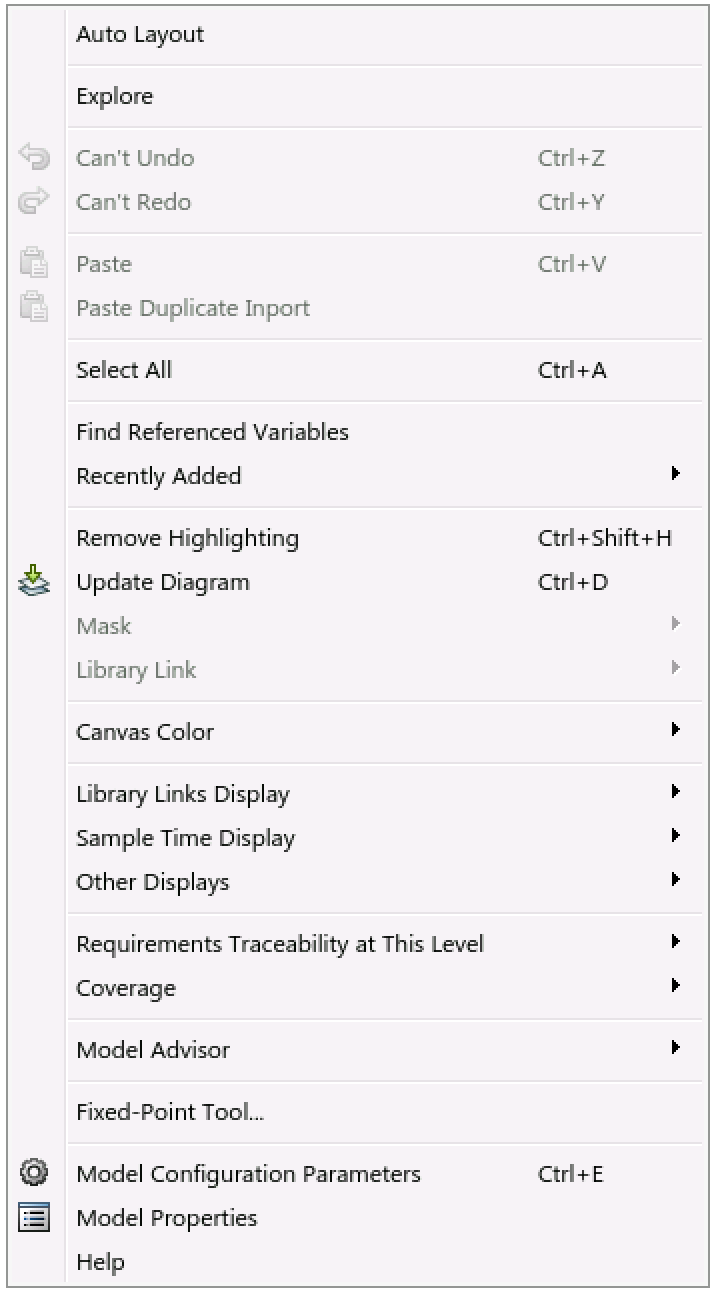
\includegraphics[width=0.63\textwidth]{../figs/ContextMenu}
	\caption{Simulink Context Menu with tool option visible.}
	\label{FIG:contextMenu}
\end{figure}

%---------------------------------------
% What are the main uses of the tool?
%---------------------------------------
\subsection{Functionality}

This section describes the tool functionality when being used from the \Simulink Context Menu (Figure~\ref{FIG:contextMenu}).

Right-clicking anywhere in the model and then selecting \cmd{\menu{1}} from the Context Menu will begin the auto layout of a model. 
If no objects are selected, the tool will act as though all objects in the system are selected.
This operation may take a few seconds.

\paragraph{\textit{Note:}} There is currently no support to undo an auto layout operation. You will be warned if you attempt to auto layout an unsaved model (Section~\ref{sec:errorwarning}).

%---------------------------------------
% What are the configuration options for the tool?
%---------------------------------------
\subsection{Configuration Parameters}
\label{SEC:config}
The configuration file \cmd{config.txt} is included in \cmd{\toolFolder\textbackslash src}. The following configuration parameters are utilized by the tool, and can be modified by the user in order to tailor tool functionality:

\begin{itemize}
	\item \label{item:layout-type} \cmd{layout\_type} -- Customize which layout method to use.
	\item \cmd{portless\_rule} -- Customize where to place blocks with no ports.
	\item \cmd{sort\_portless} -- Customize how to group blocks with no ports.
	\item \cmd{inport\_rule} -- Customize where to place inport blocks.
	\item \cmd{outport\_rule} -- Customize where to place outport blocks.
	\item \cmd{note\_rule} -- Customize where to place annotations.
	\item \cmd{show\_names} -- Customize how to show block names. 
\end{itemize}

Please see the configuration file for more details regarding parameter usage and accepted values. These parameters can be modified with \Matlab open, and do not require that \Matlab be restarted for the changes to take effect.
\\\\
There are also many configuration options available when running the tool through the command line (in addition to the configuration options). Many of these are useful for adjusting the layout slightly. A partial list of the parameters is given below:

\begin{itemize}
  \item \cmd{ShiftAll} -- Allows unselected objects to be moved out of the way as necessary when other objects are laid out.
  \item \cmd{ColumnWidthMode} -- Determines how much space to give each column of blocks in the layout.
  \item \cmd{HorizSpacing} -- Determines how much space to give between columns of blocks.
  \item \cmd{VertSpacing} -- Determines how much space to allow between blocks within a column of blocks.
  \item \cmd{AdjustWidthParams} -- Provides options pertaining to the width of blocks. (\eg a buffer to add to a width determined by the tool and whether, or not to use preset widths for certain block types).
  \item \cmd{AdjustHeightParams} -- Provides options pertaining to the height of blocks. (\eg wether or not to use preset heights for certain block types, whether or not to make blocks as tall as the sum of heights of their inputs/outputs, height desired per port, or buffer height to add to the height).
\end{itemize}

Please see \file{AutoLayout.m} in \file{\toolFolder\textbackslash src} for more details regarding usage of these parameters.

%---------------------------------------
% What else does the tool do?
%---------------------------------------
\subsection{Errors and Warnings}
\label{sec:errorwarning}
Any errors or warnings during tool use will be visible in the \Matlab Command Window. Typically, errors will be shown when the model is locked or function parameters are incorrect.

A common error occurs when one tries to start the auto layout operation on an unsaved model. As a result, the warning shown in Figure~\ref{FIG:warning} will appear. The user is given three options:
\begin{enumerate}
	\item Press \emph{Yes} to save and continue with the auto layout of the model.
	\item Press \emph{No} to continue with the auto layout of the model without saving. You may lose changes if you decide you do not wish to save after the auto layout operation.
	\item Press \emph{Cancel} or the close window button to abort the operation.
\end{enumerate}

Another common error occurs when invalid parameters or values are given when using \ToolName from the command line.
These errors are likely caused from typing in the parameter names or values incorrectly (though they should be case insensitive); it is recommended that the user review the appropriate documentation on the parameter (which should be in the header comments of the file where the error occurred).

\begin{figure}[!ht]
	\centering
	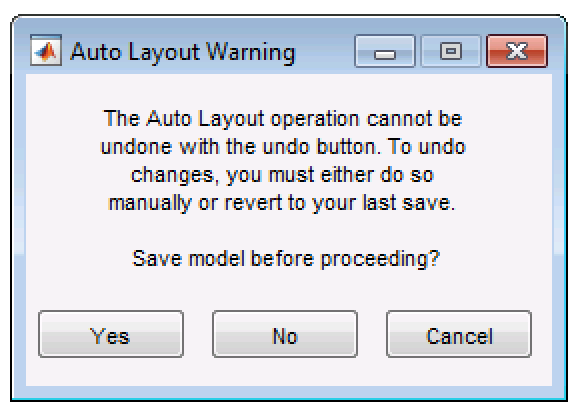
\includegraphics[width=0.5\textwidth]{../figs/Warning}
	\caption{Unsaved model warning.}
	\label{FIG:warning}
\end{figure}

\subsection{Limitations}
\label{sec:limitations}
Currently the \ToolName does not support SimScape blocks.

%%%%%%%%%%%%%%%%%%%%%%%%%%%%%%%%%%%%%%%%%%%%%%%%%%%%%%%%%%%%%%%%%%%
% Example
%%%%%%%%%%%%%%%%%%%%%%%%%%%%%%%%%%%%%%%%%%%%%%%%%%%%%%%%%%%%%%%%%%%
\section{Example}

Use the command \demoName in the \Simulink command window to open the example model, shown in Figure~\ref{FIG:demo1}. This example has many blocks that are not placed in an organized fashion, with unclear flow of data from left to right. Many signal lines are also crossing one another, making the data flow even more difficult to understand.

\begin{figure}[!ht]
	\centering
	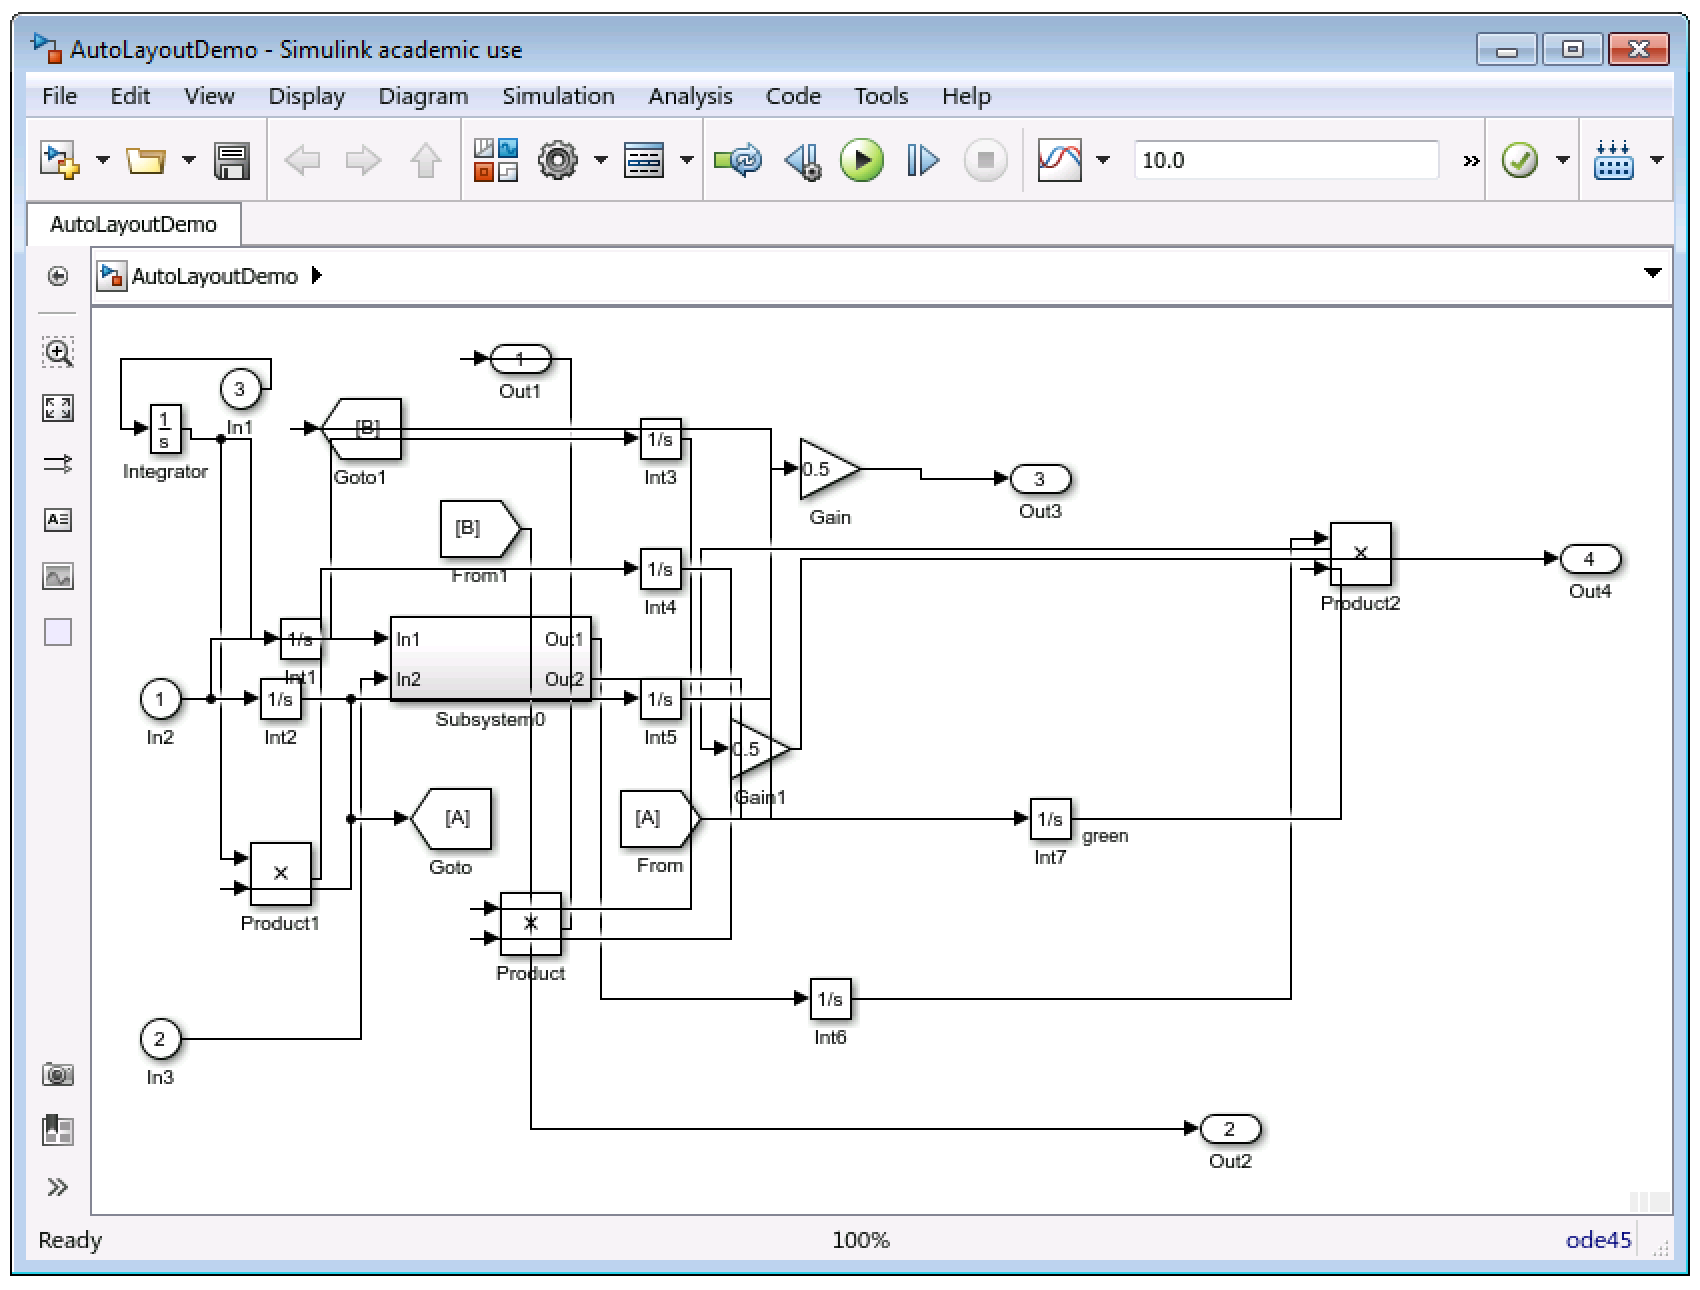
\includegraphics[width=\textwidth]{../figs/Demo1}
	\caption{\ToolName demo: The \demoName model before the auto layout operation.}
	\label{FIG:demo1}
\end{figure}

To auto layout this model, right-click anywhere in the model and select the \cmd{\menu{1}} option. The resulting model is shown in Figure~\ref{FIG:demo2}. The results will vary depending on which graphing method is used.

\begin{figure}[!ht]
	\centering
	 \begin{subfigure}[b]{0.5\textwidth}
	 	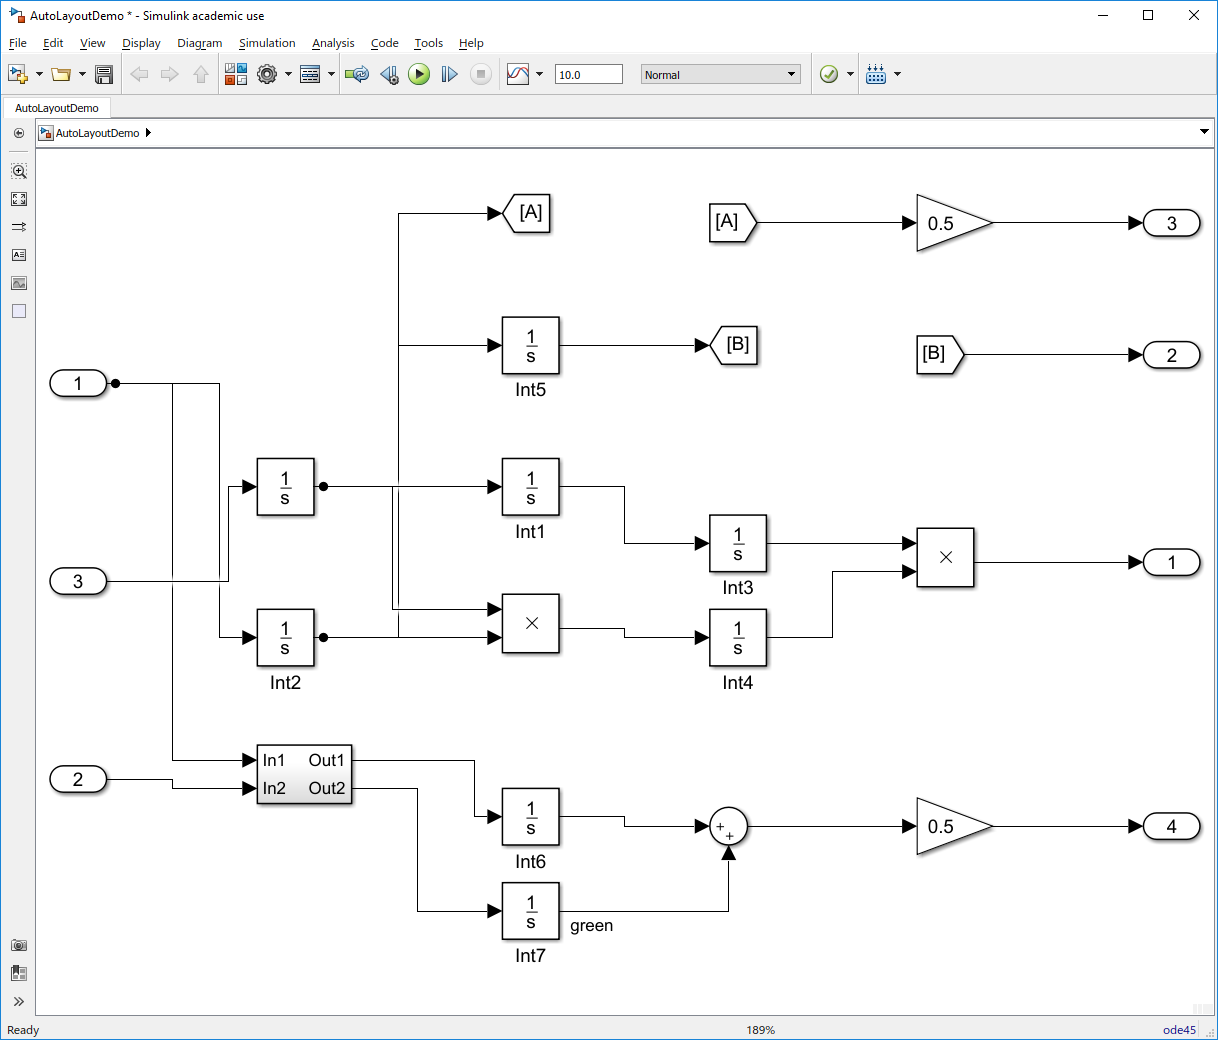
\includegraphics[width=\textwidth]{../figs/Demo2_Graphviz}
	 	\caption{Using Graphviz}
	 \end{subfigure}
	 \begin{subfigure}[b]{0.5\textwidth}
	 	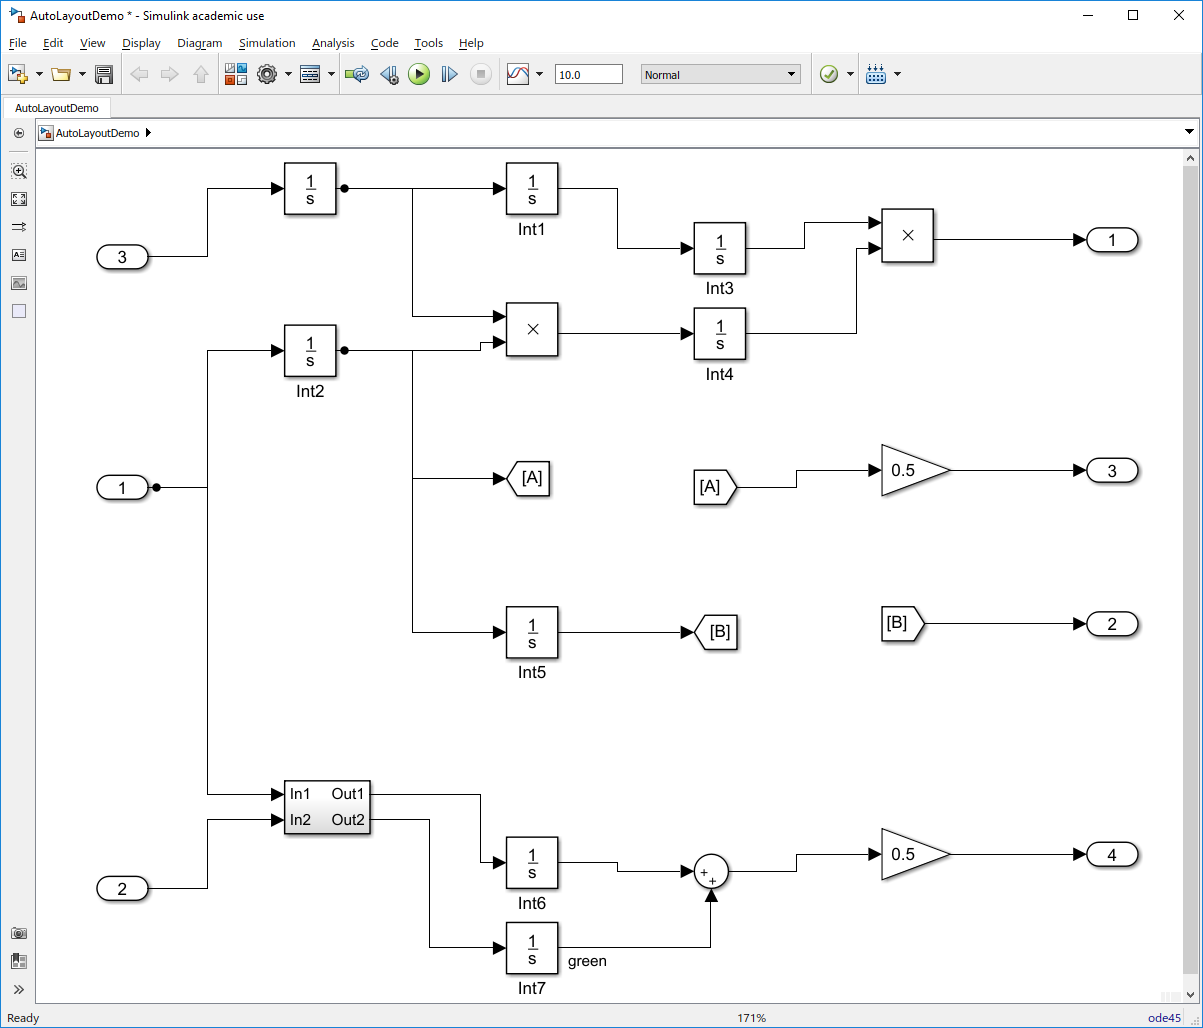
\includegraphics[width=\textwidth]{../figs/Demo2_Graphplot}
	 	\caption{Using Matlab graph plotting}
	 \end{subfigure}
	 \begin{subfigure}[b]{0.5\textwidth}
	 	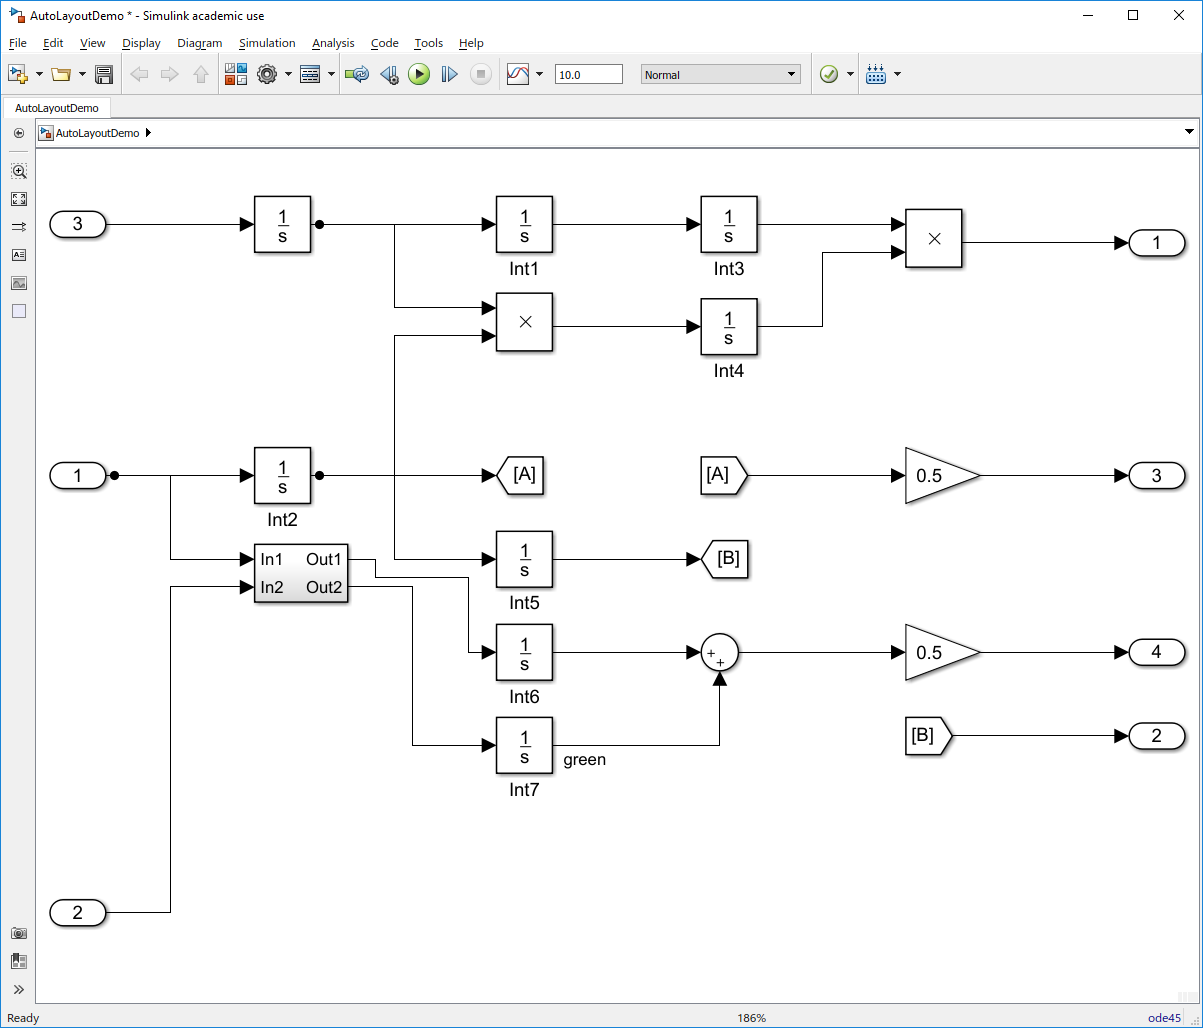
\includegraphics[width=\textwidth]{../figs/Demo2_DepthBased}
	 	\caption{Using in-house graphing method}
	 \end{subfigure}
		
	\caption{\ToolName demo: The \demoName model after the auto layout operation.}
	\label{FIG:demo2}
\end{figure}

%%%%%%%%%%%%%%%%%%%%%%%%%%%%%%%%%%%%%%%%%%%%%%%%%%%%%%%%%%%%%%%%%%%
% Matlab Commands
%%%%%%%%%%%%%%%%%%%%%%%%%%%%%%%%%%%%%%%%%%%%%%%%%%%%%%%%%%%%%%%%%%%
\clearpage
\section{Matlab Commands}

The tool can also be used via the \Matlab command line, with the following functions.
Note \cmd{gcbs} and \cmd{gcos} are useful functions that come with the tool and get the current selection of blocks and objects respectively.

%---------------------------------------
% Command 1
%---------------------------------------
\begin{center}
	\begin{tabular}{| >{\columncolor[gray]{0.9}}l | p{10.5cm} |} \hline
		Function 		& \cmd{\func{1}} \\ \hline
		Syntax			& \cmd{\func{1}}(\args{objects}, \args{varargin}) \\ \hline
		Description		& Modifies the \args{objects} within a common Simulink system so they are laid out to be more visually organized. \\ \hline
		Inputs			& \args{objects}: Simulink object (in particular: blocks \& annotations) fullnames or handles. \\ 
								& \args{varargin}: Layout options (see \file{AutoLayout.m}) \\\hline
		Outputs			& N/A \\ \hline
		Examples		& \cmd{AutoLayout(gcbs)} \\
						& \cmd{AutoLayout(gcbs, `HorizSpacing', 70)} \\
						& \cmd{AutoLayout(gcos, `HorizSpacing', 70,... `AdjustWidthParams', \{`Buffer', 10\})} \\
						& \cmd{AutoLayout(gcos, `AdjustHeightParams', \{`PortParams',... \{`ConnectionType', \{`Inport'\}, `Method', `SumMax'\}\})} \\ \hline
	\end{tabular}
\end{center}

%---------------------------------------
% Command 2
%---------------------------------------
\begin{center}
	\begin{tabular}{| >{\columncolor[gray]{0.9}}l | p{10.5cm} |} \hline
		Function 		& \cmd{\func{2}} \\ \hline
		Syntax			& \cmd{\func{2}}(\args{system}) \\ \hline
		Description		& Modifies the \args{system} model so it is laid out to be more visually organized. 
						This is the same as calling \cmd{\func{1}} with all objects in the \args{system} as input.
						\\ \hline
		Inputs			& \args{system}: Simulink system name. \\ \hline
		Outputs			& N/A\\ \hline	
	\end{tabular}
\end{center}

\end{document}